% Vector adaptation of the historical decimal -> encoded -> delta-matrix figure.
% Illustration only: exact INT8, affine scale 1/16, zero point 0.
% Columns are b7 (two's-complement sign) through b0, from left to right.
\begingroup%
\definecolor{deltaInk}{HTML}{18354A}%
\definecolor{deltaBlue}{HTML}{9BC9DE}%
\definecolor{deltaRose}{HTML}{D58EA6}%
\definecolor{deltaGreen}{HTML}{A3D5B1}%
\definecolor{deltaSign}{HTML}{A83D5B}%
\definecolor{deltaBit}{HTML}{087E8B}%
\resizebox{\linewidth}{!}{%
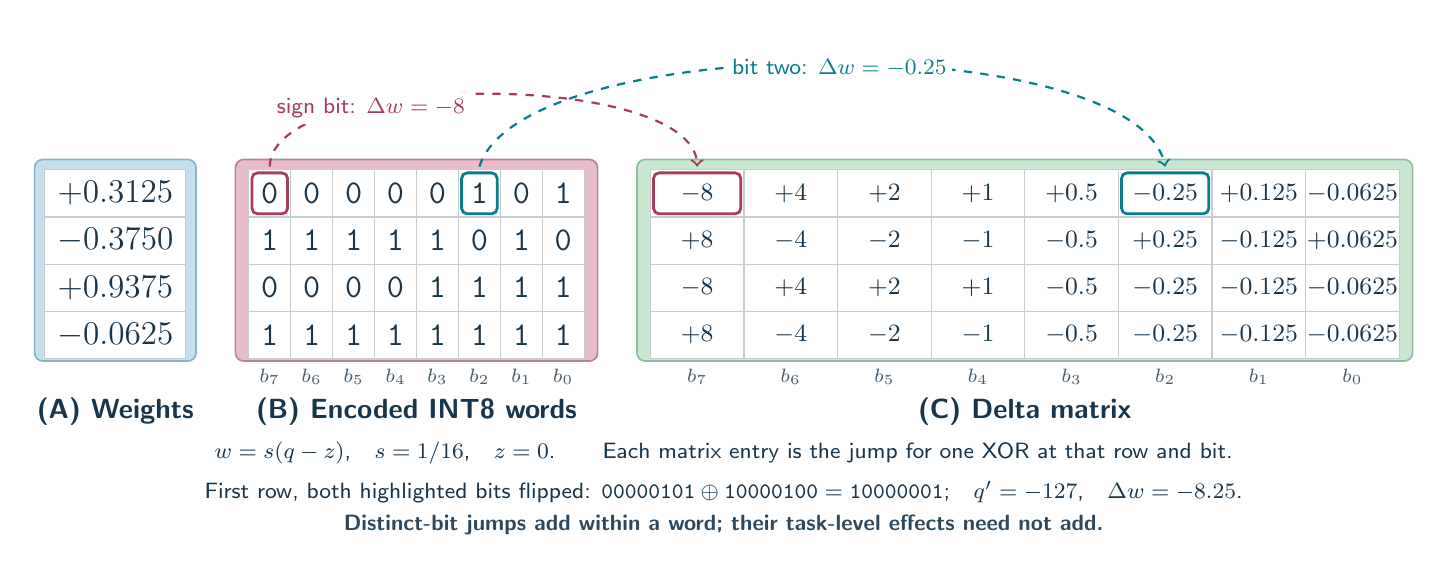
\begin{tikzpicture}[font=\sffamily\small,text=deltaInk]
  % The three colored frames deliberately retain the old paper's visual grammar.
  \draw[rounded corners=3pt,draw=deltaBlue!85!deltaInk,fill=deltaBlue!58,line width=.6pt]
    (0,0) rectangle (2.05,2.56);
  \draw[rounded corners=3pt,draw=deltaRose!85!deltaInk,fill=deltaRose!58,line width=.6pt]
    (2.55,0) rectangle (7.15,2.56);
  \draw[rounded corners=3pt,draw=deltaGreen!85!deltaInk,fill=deltaGreen!58,line width=.6pt]
    (7.65,0) rectangle (17.50,2.56);

  % Decoded values. Every allocated word remains present, regardless of value.
  \foreach \row/\value in {0/{+0.3125},1/{-0.3750},2/{+0.9375},3/{-0.0625}}{
    \draw[draw=deltaInk!25,fill=white] (.13,2.43-\row*.60) rectangle (1.92,1.83-\row*.60);
    \node[font=\sffamily\large] at (1.025,2.13-\row*.60) {$\value$};
  }

  % Encoded INT8 words, MSB at left: 5, -6, 15 and -1.
  \foreach \row/\word in {0/{0,0,0,0,0,1,0,1},1/{1,1,1,1,1,0,1,0},2/{0,0,0,0,1,1,1,1},3/{1,1,1,1,1,1,1,1}}{
    \foreach \digit [count=\col from 0] in \word {
      \draw[draw=deltaInk!25,fill=white] (2.72+\col*.5325,2.43-\row*.60)
        rectangle (3.2525+\col*.5325,1.83-\row*.60);
      \node[font=\ttfamily\large] at (2.98625+\col*.5325,2.13-\row*.60) {\digit};
    }
  }

  % Exact single-bit jumps s(q' - q), in the same MSB-to-LSB column order.
  \foreach \row/\jumps in {0/{-8,+4,+2,+1,+0.5,-0.25,+0.125,-0.0625},1/{+8,-4,-2,-1,-0.5,+0.25,-0.125,+0.0625},2/{-8,+4,+2,+1,-0.5,-0.25,-0.125,-0.0625},3/{+8,-4,-2,-1,-0.5,-0.25,-0.125,-0.0625}}{
    \foreach \jump [count=\col from 0] in \jumps {
      \draw[draw=deltaInk!25,fill=white] (7.82+\col*1.18875,2.43-\row*.60)
        rectangle (9.00875+\col*1.18875,1.83-\row*.60);
      \node at (8.414375+\col*1.18875,2.13-\row*.60) {$\jump$};
    }
  }

  % Color-linked single-bit transitions in the first row, as in the original.
  \draw[deltaSign,line width=1pt,rounded corners=2pt]
    (2.76,1.87) rectangle (3.2125,2.39);
  \draw[deltaSign,line width=1pt,rounded corners=2pt]
    (7.86,1.87) rectangle (8.96875,2.39);
  \draw[deltaBit,line width=1pt,rounded corners=2pt]
    (5.4225,1.87) rectangle (5.875,2.39);
  \draw[deltaBit,line width=1pt,rounded corners=2pt]
    (13.80375,1.87) rectangle (14.9125,2.39);
  \draw[->,deltaSign,line width=.8pt,dashed]
    (2.98625,2.47) .. controls (3.00,3.70) and (8.40,3.70) .. (8.414375,2.47);
  \draw[->,deltaBit,line width=.8pt,dashed]
    (5.64875,2.47) .. controls (6.20,4.22) and (14.00,4.22) .. (14.358125,2.47);
  \node[fill=white,inner sep=2pt,text=deltaSign,font=\sffamily\footnotesize]
    at (4.27,3.21) {sign bit: $\Delta w=-8$};
  \node[fill=white,inner sep=2pt,text=deltaBit,font=\sffamily\footnotesize]
    at (10.22,3.72) {bit two: $\Delta w=-0.25$};

  % Bit indices under the two matrices make the storage convention explicit.
  \foreach \col/\bit in {0/7,1/6,2/5,3/4,4/3,5/2,6/1,7/0}{
    \node[font=\sffamily\scriptsize,text=deltaInk!80] at (2.98625+\col*.5325,-.20) {$b_{\bit}$};
    \node[font=\sffamily\scriptsize,text=deltaInk!80] at (8.414375+\col*1.18875,-.20) {$b_{\bit}$};
  }
  \node[font=\sffamily\bfseries] at (1.025,-.64) {(A) Weights};
  \node[font=\sffamily\bfseries] at (4.85,-.64) {(B) Encoded INT8 words};
  \node[font=\sffamily\bfseries] at (12.575,-.64) {(C) Delta matrix};
  \node[font=\sffamily\footnotesize,align=center] at (8.75,-1.17)
    {$w=s(q-z)$,\quad $s=1/16$,\quad $z=0$.\qquad Each matrix entry is the jump for one XOR at that row and bit.};
  \node[font=\sffamily\footnotesize,align=center] at (8.75,-1.66)
    {First row, both highlighted bits flipped: $\mathtt{00000101}\oplus\mathtt{10000100}=\mathtt{10000001}$;\quad $q'=-127$,\quad $\Delta w=-8.25$.};
  \node[font=\sffamily\footnotesize\bfseries,text=deltaInk!90] at (8.75,-2.08)
    {Distinct-bit jumps add within a word; their task-level effects need not add.};
\end{tikzpicture}%
}%
\endgroup%
